\documentclass{article}
\usepackage{ctex}
\usepackage{graphicx}
\usepackage{subcaption}
\usepackage{wrapfig}
\usepackage[colorlinks = true,linkcolor=blue]{hyperref}

%* 以下插入的图片外面都套有一层"\fbox{text}"命令,以清楚显示图片的边框界限

\begin{document}

\tableofcontents

\newpage

\section{图片原始大小}
% graphicx宏包命令
    %picture in the same file as Tex
    \fbox{\includegraphics{doraemon1.jpg}}
    % XeLaTeX支持pdf、eps、png与jpg图片扩展名,所以可以写带扩展名的图片名称,也可以写不带扩展名的名称,如果不给出扩展名,将按上述4个扩展名的顺序依次搜索文件(吴康隆P50)

    % 绝对路径
    % \includegraphics{D:/OneDrive/(▲)Yuanhao_github/Yuanhao_LaTeX_github/Test/LaTeX_Picture/doraemon1.jpg} 
    %? 使用相对路径始终无法成功编译,不知道原因是什么

    %reserved file for pictures
    % \graphicspath{{D:/OneDrive/(▲)Yuanhao_github/Yuanhao_LaTeX_github/Test/LaTeX_Picture/Reserved file for pictures}}
    % 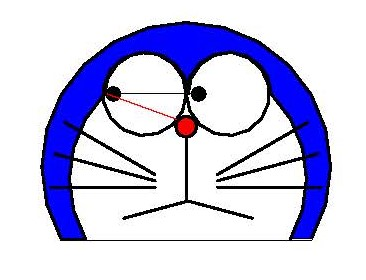
\includegraphics{doraemon2.jpg}
    %* 注意,使用"\graphicspath{dir-list}"命令时,路径两边应该套用两层大括号,否则无法成功编译

\section{scale表示图片缩放倍数(0.3倍/0.5倍/0.7倍)}
    \fbox{\includegraphics[scale=.3]{doraemon1.jpg}}
    \fbox{\includegraphics[scale=.5]{doraemon1.jpg}}
    \fbox{\includegraphics[scale=.7]{doraemon1.jpg}}

\section{width表示图片宽度(3cm/0.3倍页宽)}

    \fbox{\includegraphics[width=3cm]{doraemon1.jpg}}
    \fbox{\includegraphics[width=.3\textwidth]{doraemon1.jpg}}

\section{height表示图片高度(1cm/0.1倍页高)}
    % 旋转的图片基线会变化,故一般用totalheight代替height(吴康隆P50)
    \fbox{\includegraphics[height=1cm]{doraemon1.jpg}}
    \fbox{\includegraphics[height=.1\textheight]{doraemon1.jpg}}

\section{angle表示图片逆时针旋转角度,origin表示图片旋转中心,默认值为l(左),可以设置为r(右)、c(中)、t(顶)、b(底)、B(基线)}
%* 顺时针旋转可以通过在旋转角度前面添加符号来完成
\subsection{绕左侧中心逆时针旋转90度}
    \fbox{\includegraphics[angle=90]{doraemon1.jpg}}%counterclockwise
    \fbox{\includegraphics{doraemon1.jpg}}

\subsection{绕左侧中心顺时针旋转90度}
    \fbox{\includegraphics[angle=-90]{doraemon1.jpg}}%clockwise
    \fbox{\includegraphics{doraemon1.jpg}}

\subsection{绕右侧中心逆时针旋转90度}
    \fbox{\includegraphics{doraemon1.jpg}}
    \fbox{\includegraphics[angle=90, origin=r]{doraemon1.jpg}}

\subsection{绕中央中心逆时针旋转90度}
    \fbox{\includegraphics{doraemon1.jpg}}
    \fbox{\includegraphics[angle=90, origin=c]{doraemon1.jpg}}

\subsection{绕中心顶端中心逆时针旋转90度}
    \fbox{\includegraphics{doraemon1.jpg}}
    \fbox{\includegraphics[angle=90, origin=t]{doraemon1.jpg}}

\subsection{绕底部中心逆时针旋转90度}
    \fbox{\includegraphics{doraemon1.jpg}}
    \fbox{\includegraphics[angle=90, origin=b]{doraemon1.jpg}}

\subsection{绕基线中心逆时针旋转90度}
    \fbox{\includegraphics{doraemon1.jpg}}
    \fbox{\includegraphics[angle=90, origin=B]{doraemon1.jpg}}

\section{设置图片到边框的距离(原始尺寸/0.5cm)}
    \fbox{\includegraphics{doraemon1.jpg}}
    \setlength{\fboxsep}{.5cm}
    \fbox{\includegraphics{doraemon1.jpg}}

\section{在文本中插入图片}
\subsection{不使用浮动体环境}
    This is a picture \fbox{\includegraphics{doraemon1.jpg}} inserted into the text.

\subsection{使用浮动体环境}
    This is a picture independent of the text.
    \begin{figure}[htbp]
        \centering
        \fbox{\includegraphics{doraemon1.jpg}}
        \caption{doraemon\_figure}
    \end{figure}

% subcaption宏包命令
    \begin{figure}[htbp]
        \centering
        \begin{subfigure}{.3\textwidth}%this argument of width is obligatory
            \centering
            \fbox{\includegraphics[scale=.1]{doraemon1.jpg}}
            \subcaption{doraemon (1)}
        \end{subfigure}
        %
        \begin{subfigure}{.3\textwidth}
            \centering
            \fbox{\includegraphics[scale=.3]{doraemon1.jpg}}
            \subcaption{doraemon (2)}
        \end{subfigure}
        %
        \begin{subfigure}{.3\textwidth}
            \centering
            \fbox{\includegraphics[scale=.5]{doraemon1.jpg}}
            \caption{doraemon (3)} % subfigure环境中既可以使用"\subcaption{}"命令,也可以使用"\caption{}"命令
        \end{subfigure}	
        \caption{doraemon\_subfigure}	
    \end{figure}

% \clearpage
%rfr 使用"\clearpage"命令来清空浮动队列,并且新开一页,如果此处不使用这一项命令,则"doraemon_subfigure"一图会作为浮动体被插入到下面的文本当中,关于"\newpage"命令和"\clearpage"命令的区别,可以参考:https://blog.csdn.net/weixin_45008608/article/details/115835064、https://www.latexstudio.net/archives/8005.html

\section{图文混排}
% wrapfig宏包命令
    Texte texte texte texte texte texte texte
    texte texte texte texte texte texte texte
    texte texte texte texte texte texte...
    Texte texte texte texte texte texte texte
    texte texte texte texte texte texte texte
    texte texte texte texte texte texte...

    \begin{wrapfigure}{l}{5cm}%Notice that this is the argument of width
        \centering
        \fbox{\includegraphics[scale=.3]{doraemon1.jpg}}
        \caption{doraemon\_wrapfigure}
    \end{wrapfigure}
    Texte texte texte texte texte texte texte
    texte texte texte texte texte texte texte
    texte texte texte texte texte texte...
    Texte texte texte texte texte texte texte
    texte texte texte texte texte texte texte
    texte texte texte texte texte texte...
    Texte texte texte texte texte texte texte
    texte texte texte texte texte texte texte
    texte texte texte texte texte texte...
    Texte texte texte texte texte texte texte
    texte texte texte texte texte texte texte
    texte texte texte texte texte texte...
    % wrapfigure环境有两个必选参数,两个可选参数:[linenum]{place}[overhang]{picwidth},必选参数包括{place}和{picwidth},{place}可以选择r、l、i、o,分别代表图片在文字段的左侧、右侧、近书脊、远书脊,{picwidth}代表图片的宽度,图片的高度会自动调整;可选参数包括[linenum]和[overhang],[linenum]代表图片所占行数,一般不指定,[overhang]代表允许图片超出页面文本区的宽度,默认是0pt,即不允许图片超出页面文本区,该项可以使用"\width"代替图片的宽度,填入"\width"将允许把图片全部放入页边区域(吴康隆P51)

\listoffigures
%* 插图目录显示所有在浮动体环境中使用"\caption{heading}"命令对应的图片所在页码
\end{document}